\documentclass[../main.tex]{subfiles}
\begin{document}

As part of our project, we implemented two fully instrumented FaaS based demo applications:
An e-commerce application (i.e.\@ a webshop) and an IoT-resembling traffic light calculator for some road crossing.
They serve both as examples how to build fully working and adaptively deployable applications 
within our framework as well as a baseline for real application-oriented FaaS benchmarks.

\section{E-Commerce Application (Webshop)}\label{sec:webshop}

% Design Concepts
We implemented a test e-commerce application that fully consists of FaaS components together with a redis database. 
The basic functionality is to display recommended products and ads to customers 
who can then buy said products by charging a mocked credit card. 
As such, the deployed application can theoretically be ``used'' exclusively by humans 
interacting with its website frontend within a web browser.
Naturally, there are also pre-defined automatized workloads to secure a benchmark's reproducibility.

\subsection{Application Design}\label{ssec:webshopApplicationStructure}

The webshop's functionality is closely oriented on Google’s microservices demo v0.1.0\footnotemark{} 
but has of course been fully reimplemented as a FaaS project 
(except for some HTML templates as visible in the frontend function's source code directory). 
\footnotetext{\url{https://github.com/GoogleCloudPlatform/microservices-demo/tree/bae651f7ea537d2676b38a04d89adacdd45c17bd}}

\begin{figure}[]
\begin{center}
  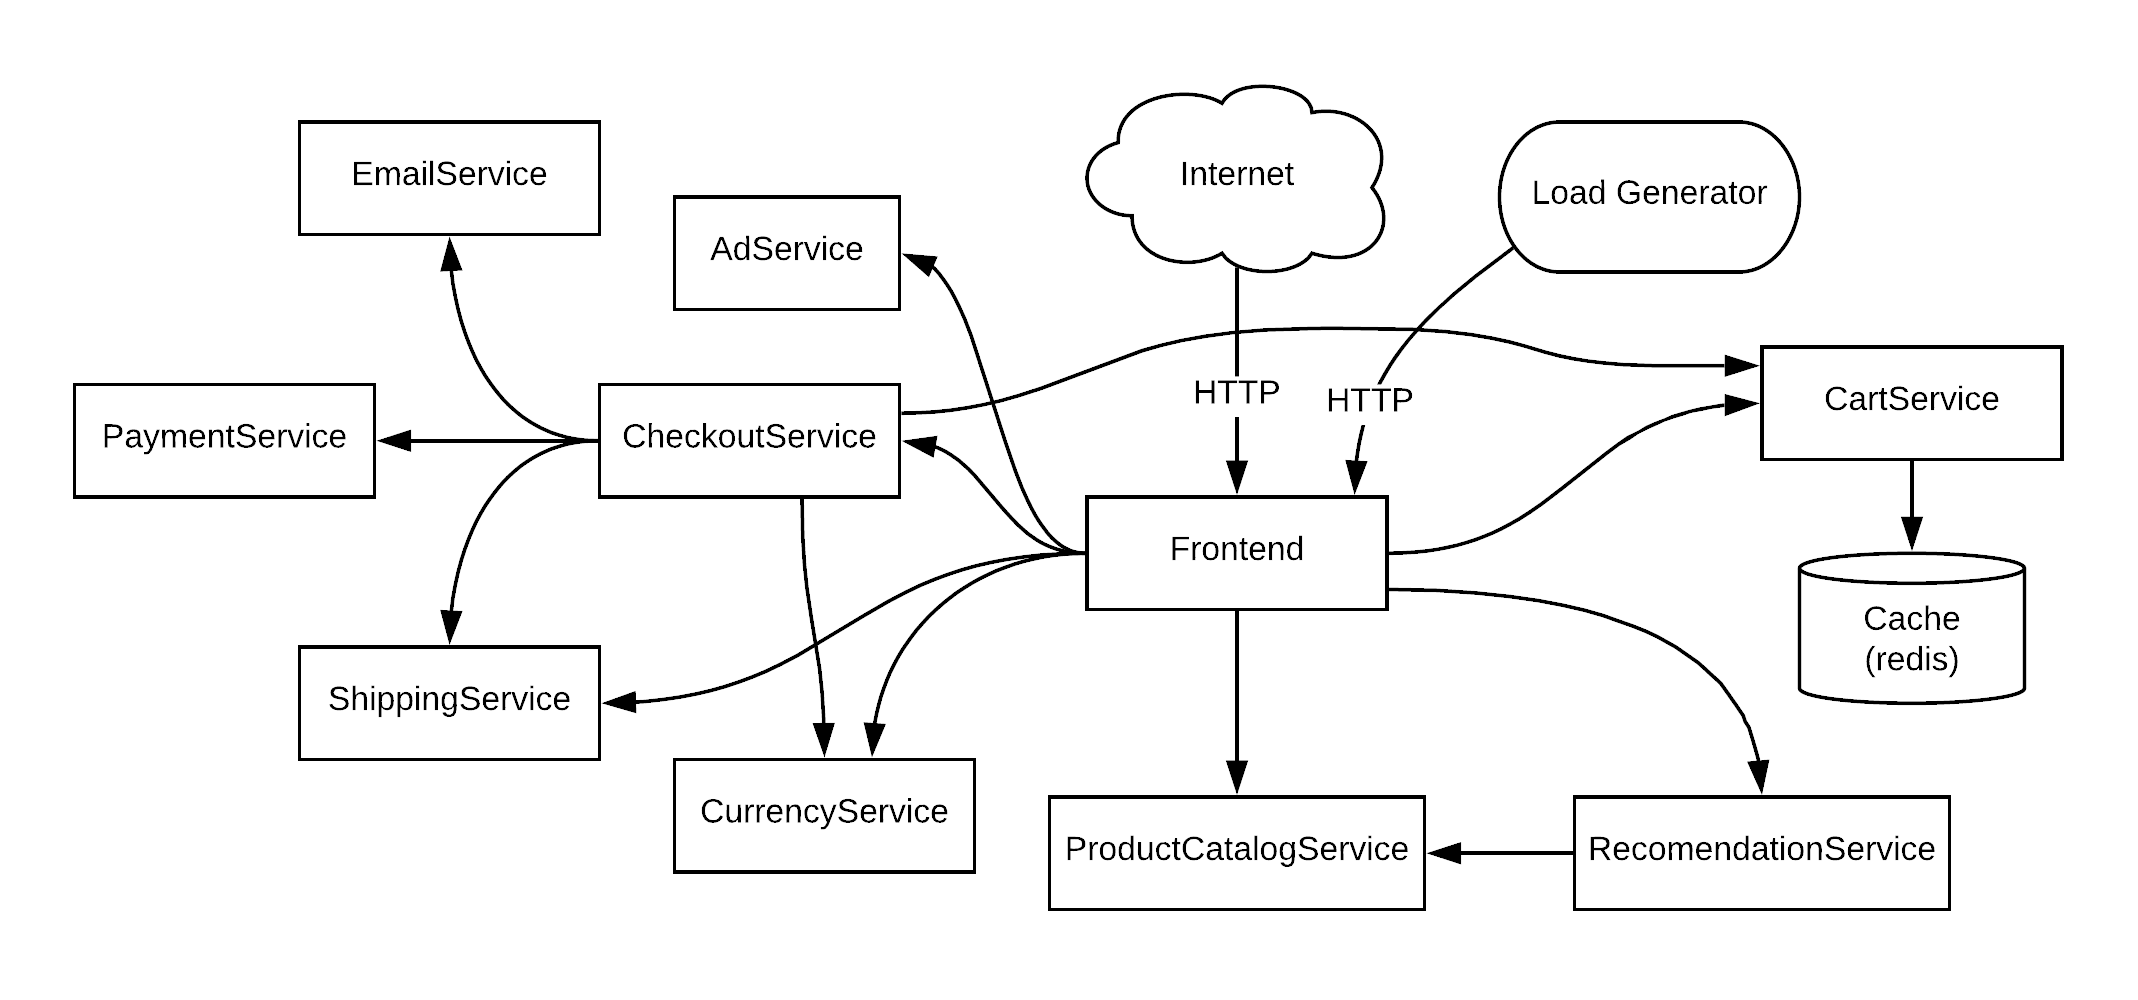
\includegraphics[width=\linewidth,keepaspectratio]{./webshop-architecture-diagram.png}
\end{center}
\caption[Webshop Architecture Diagram]{%
  Webshop architecture diagram as illustrated by Google\protect\footnotemark.
  %TODO remove external API
  All `services' as well as the frontend are implemented as separate functions within our demo application. 
  They communicate internally with each other via our library's RPC system and are thus automatically measured at runtime.%
}%
\label{fig:webshopArchitectureDiagram}
\end{figure}
\footnotetext{\url{https://raw.githubusercontent.com/GoogleCloudPlatform/microservices-demo/bae651f7ea537d2676b38a04d89adacdd45c17bd/docs/img/architecture-diagram.png}}

Google's architecture diagram, which also conveys the idea of our setup, can be found in \Cref{fig:webshopArchitectureDiagram}.
However as Google developed their demo to showcase the capabilities of microservices, 
their `services' often bundle the functionality of multiple callable functions by context.
True to the FaaS paradigm (one function per need), 
we usually split those functionalities into separate callable functions in our application.
\Cref{tab:webshopFunctionOverview} shows how Google's services are divided into our implemented functions.
It also outlines each function's individual purpose.

In short users may log in, browse recommended products, view ads, set their preferred currency (triggering product price conversion),
and put some items into their shopping cart (thus internally using the cart database).
Finally they can checkout their order, leading to a payment and a shipping process.

\begin{longtable}{l l l} 
  \caption[Webshop Function Overview]{Webshop Function Overview\vspace*{1mm}}\label{tab:webshopFunctionOverview}\\
  \textbf{Service} & \textbf{Function} &  \textbf{Description}\\ 
  \toprule
  %\endhead{}%
  Frontend                                & frontend            & 
  \makecell[{{p{6.5cm}}}]{Receives user requests and displays webpage. 
    Calls all other functions (except payment, email and shiporder) depending on requests.}\\
  \midrule[0.02em]
  \multirow{3}{*}{Product Catalog Service}& getproduct          &
  \makecell[{{p{6.5cm}}}]{Returns all data about a product given its ID.}\\
  \cmidrule[0.02em]{2-3}
                                          & listproducts        &
  \makecell[{{p{6.5cm}}}]{Returns all data about available products.}\\
  \cmidrule[0.02em]{2-3}
                                          & searchproducts      &
  \makecell[{{p{6.5cm}}}]{Searches product catalog for some string and 
    returns all matching products.}\\
  \midrule[0.02em]
  Recommendation Service                  & listrecommendations &
  \makecell[{{p{6.5cm}}}]{Takes a list of product IDs, responds with 
    list of up to 7 other related (`recommended') 
    product IDs.}\\
  \midrule[0.02em]
  \multirow{4}{*}{Cart Service}           & getcart             & 
  \makecell[{{p{6.5cm}}}]{Returns a given user's shopping cart.}\\
  \cmidrule[0.02em]{2-3}
                                          & addcartitem         & 
  \makecell[{{p{6.5cm}}}]{Adds an item to a user's shopping cart.}\\
  \cmidrule[0.02em]{2-3}
                                          & emptycart           & 
  \makecell[{{p{6.5cm}}}]{Empties a given user's shopping cart.}\\
  \cmidrule[0.02em]{2-3}
                                          & cartkvstorage       & 
  \makecell[{{p{6.5cm}}}]{Manages the internal cart database. 
    Only called by the other cart service functions.}\\
  \midrule[0.02em]
  Checkout Service                        & checkout            &
    \makecell[{{p{6.5cm}}}]{Handles a checkout process when requested 
    by user (via frontend). Involves e.g.\@ calling 
    payment, shiporder, email and emptycart.}\\
  \midrule[0.02em]
  \multirow{2}{*}{Currency Service}       & currency            &
  \makecell[{{p{6.5cm}}}]{Converts a price from one currency to another.}\\
  \cmidrule[0.02em]{2-3}
                                          & supportedcurrencies &
  \makecell[{{p{6.5cm}}}]{Returns a list of all supported currencies.}\\
  \midrule[0.02em]
  Payment Service                         & payment             &
  \makecell[{{p{6.5cm}}}]{Handles a payment.}\\
  \midrule[0.02em]
  \multirow{2}{*}{Shipping Service}       & shipmentquote       &
  \makecell[{{p{6.5cm}}}]{Calculates cost of shipping a given order.}\\
  \cmidrule[0.02em]{2-3}
                                          & shiporder           &
  \makecell[{{p{6.5cm}}}]{Handles actual shipping of an order.}\\
  \midrule[0.02em]
  Email Service                           & email               &
  \makecell[{{p{6.5cm}}}]{Sends a confirmation email.}\\
  \midrule[0.02em]
  Ad Service                              & getads              &
  \makecell[{{p{6.5cm}}}]{Supplies links to random cat pictures.}\\
  \bottomrule
\end{longtable}

% TODO Call Spec Appendix?
Exact Function I/O specification can also be looked up within the source code\footnotemark.
There, each function has its I/O behaviour (including individual examples) documented.
\footnotetext{\url{https://github.com/FaaSterMetrics/experiments/tree/master/experiments/webservice/functions}}

\subsection{Benchmarking Properties}\label{ssec:webshopApplicationProperties}

The most prominent feature of such this application from a benchmarking perspective is its high functional interdependence. 
Many different components are meshed and require each other as outlines 
in \Cref{fig:webshopArchitectureDiagram} and \Cref{tab:webshopFunctionOverview}.

The webshop also features a non-homogenous request system: 
Since different users' behavior is dissimilar by nature 
(some may like to browse a lot whereas others just buy everything they are recommended instantly), 
so are the various requests the webshop has to deal with simultaneously.

Other characteristic properties are a rather read-heavy behaviour in general 
(there is much required input data from various sources) 
and thus a sizable response to customers (e.g.\@ pictures, web design). 
Also, the functionality depends on a single database, representing real-world state-locking.


\subsection{Specific Workloads}\label{ssec:webshopSpecificWorkloads}

To complete the experiment, we also pre-defined some workload profiles which were automatized with \texttt{artillery}
(see \Cref{sec:sec:WorkloadsStructure}).
Obviously, each of those profiles leads to an individual experiment.
Thus, you should use the application's workload profile that reflects the situation you want to analyse the closest,
or develop your own one if required.
That said, the first described workload profile suits an average webshop scenario best and is therefore generally recommended.

\subsubsection{Average High Webshop Traffic}%
\label{ssub:webshopProfileHighTraffic}

This workload profile aims to simulate normal high traffic situations.
Many customers visit the webshop, but not everyone actually buys products.
This means that there are rather shallow and rather deep (nested) function calls in a fairly equal manner.
As such, the load on the frontend and e.g.\@ the ad service (which are always used) is in total much heavier than e.g.\@ 
on the checkout service.

In terms of resources, this workload is more CPU heavy than reliant on external I/O (database),
since many customers just browse and do not place many products into their cart (which uses the database).
It also features a gradual load increase, meaning that while functions do perform cold-start at the beginning,
those will not all happen similarly in a large quantity, since some functions will only be called later.

The profile can be found in the repository's webservice directory as 
\begin{tcolorbox}
\quad\texttt{workload-constant-high-load-uniform.yml}
\end{tcolorbox}

\subsubsection{Black Friday Advertisement}%
\label{ssub:webshopProfileBlackFridayAds}

There is a sudden new Black Friday promotion where some famous product can be bought at half price.
Links to the shop are shared all over social media and consequently there is a very sudden burst towards high traffic
within a short time period.

This profile also features many deep (nested) function calls, since the customers are all buying that one product.
Thus, in not only stress-tests elasticity capacities (triggering many cold-starts in a short time),
it also relies on the external shopping cart database rather heavily, because each customer triggers multiple database calls.

The profile can be found in the repository's webservice directory as 
\begin{tcolorbox}
\quad\texttt{workload-cold-to-spike.yml}
\end{tcolorbox}

\subsubsection{Black Friday Afternoon}%
\label{ssub:webshopProfileBlackFridayDaytime}

This workload profile is more directed at simulating an average Black Friday afternoon situation:
Very many people visit the shop, but most of them only enjoy window-shopping. 
They basically visit the shop only to compare its special offers to those of other webshops
and then just go for the other shop or none at all.

Thus, this profile is rather similar to the first (\Cref{ssub:webshopProfileHighTraffic}),
but the ratio of deep to shallow calls is much more favored towards the former.
This means, that nearly all load lies on the frontend and the functions it directly calls.
Functions like checkout, payment or even the external database are hardly used at all.

The profile can be found in the repository's webservice directory as 
\begin{tcolorbox}
\quad\texttt{workload-constant-high-load-shallow.yml}
\end{tcolorbox}

\subsubsection{Regular Morning Increase}%
\label{ssub:webshopProfileRegularMorning}

This workload profile tries to represent a regular weekday morning: 
The later it gets, the more people wake up and each one of them realizes they needed to buy exactly one product.
Thus, they go exactly for this one product only and then leave for work.

This profile is most interesting if one wants to test all functions and the database in a rather similar number.
Since each customer buys exactly one product (deep function calls, triggering whole checkout process),
all functions are used. 
Obviously, the frontend still carries a (constant times) higher load than the other functions, 
since it has to process and forward each user request.

The profile can be found in the repository's webservice directory as 
\begin{tcolorbox}
\quad\texttt{workload-phases-all-buy.yml}
\end{tcolorbox}
\end{document}
